\begin{figure}[h!]
	\adjustbox{center}{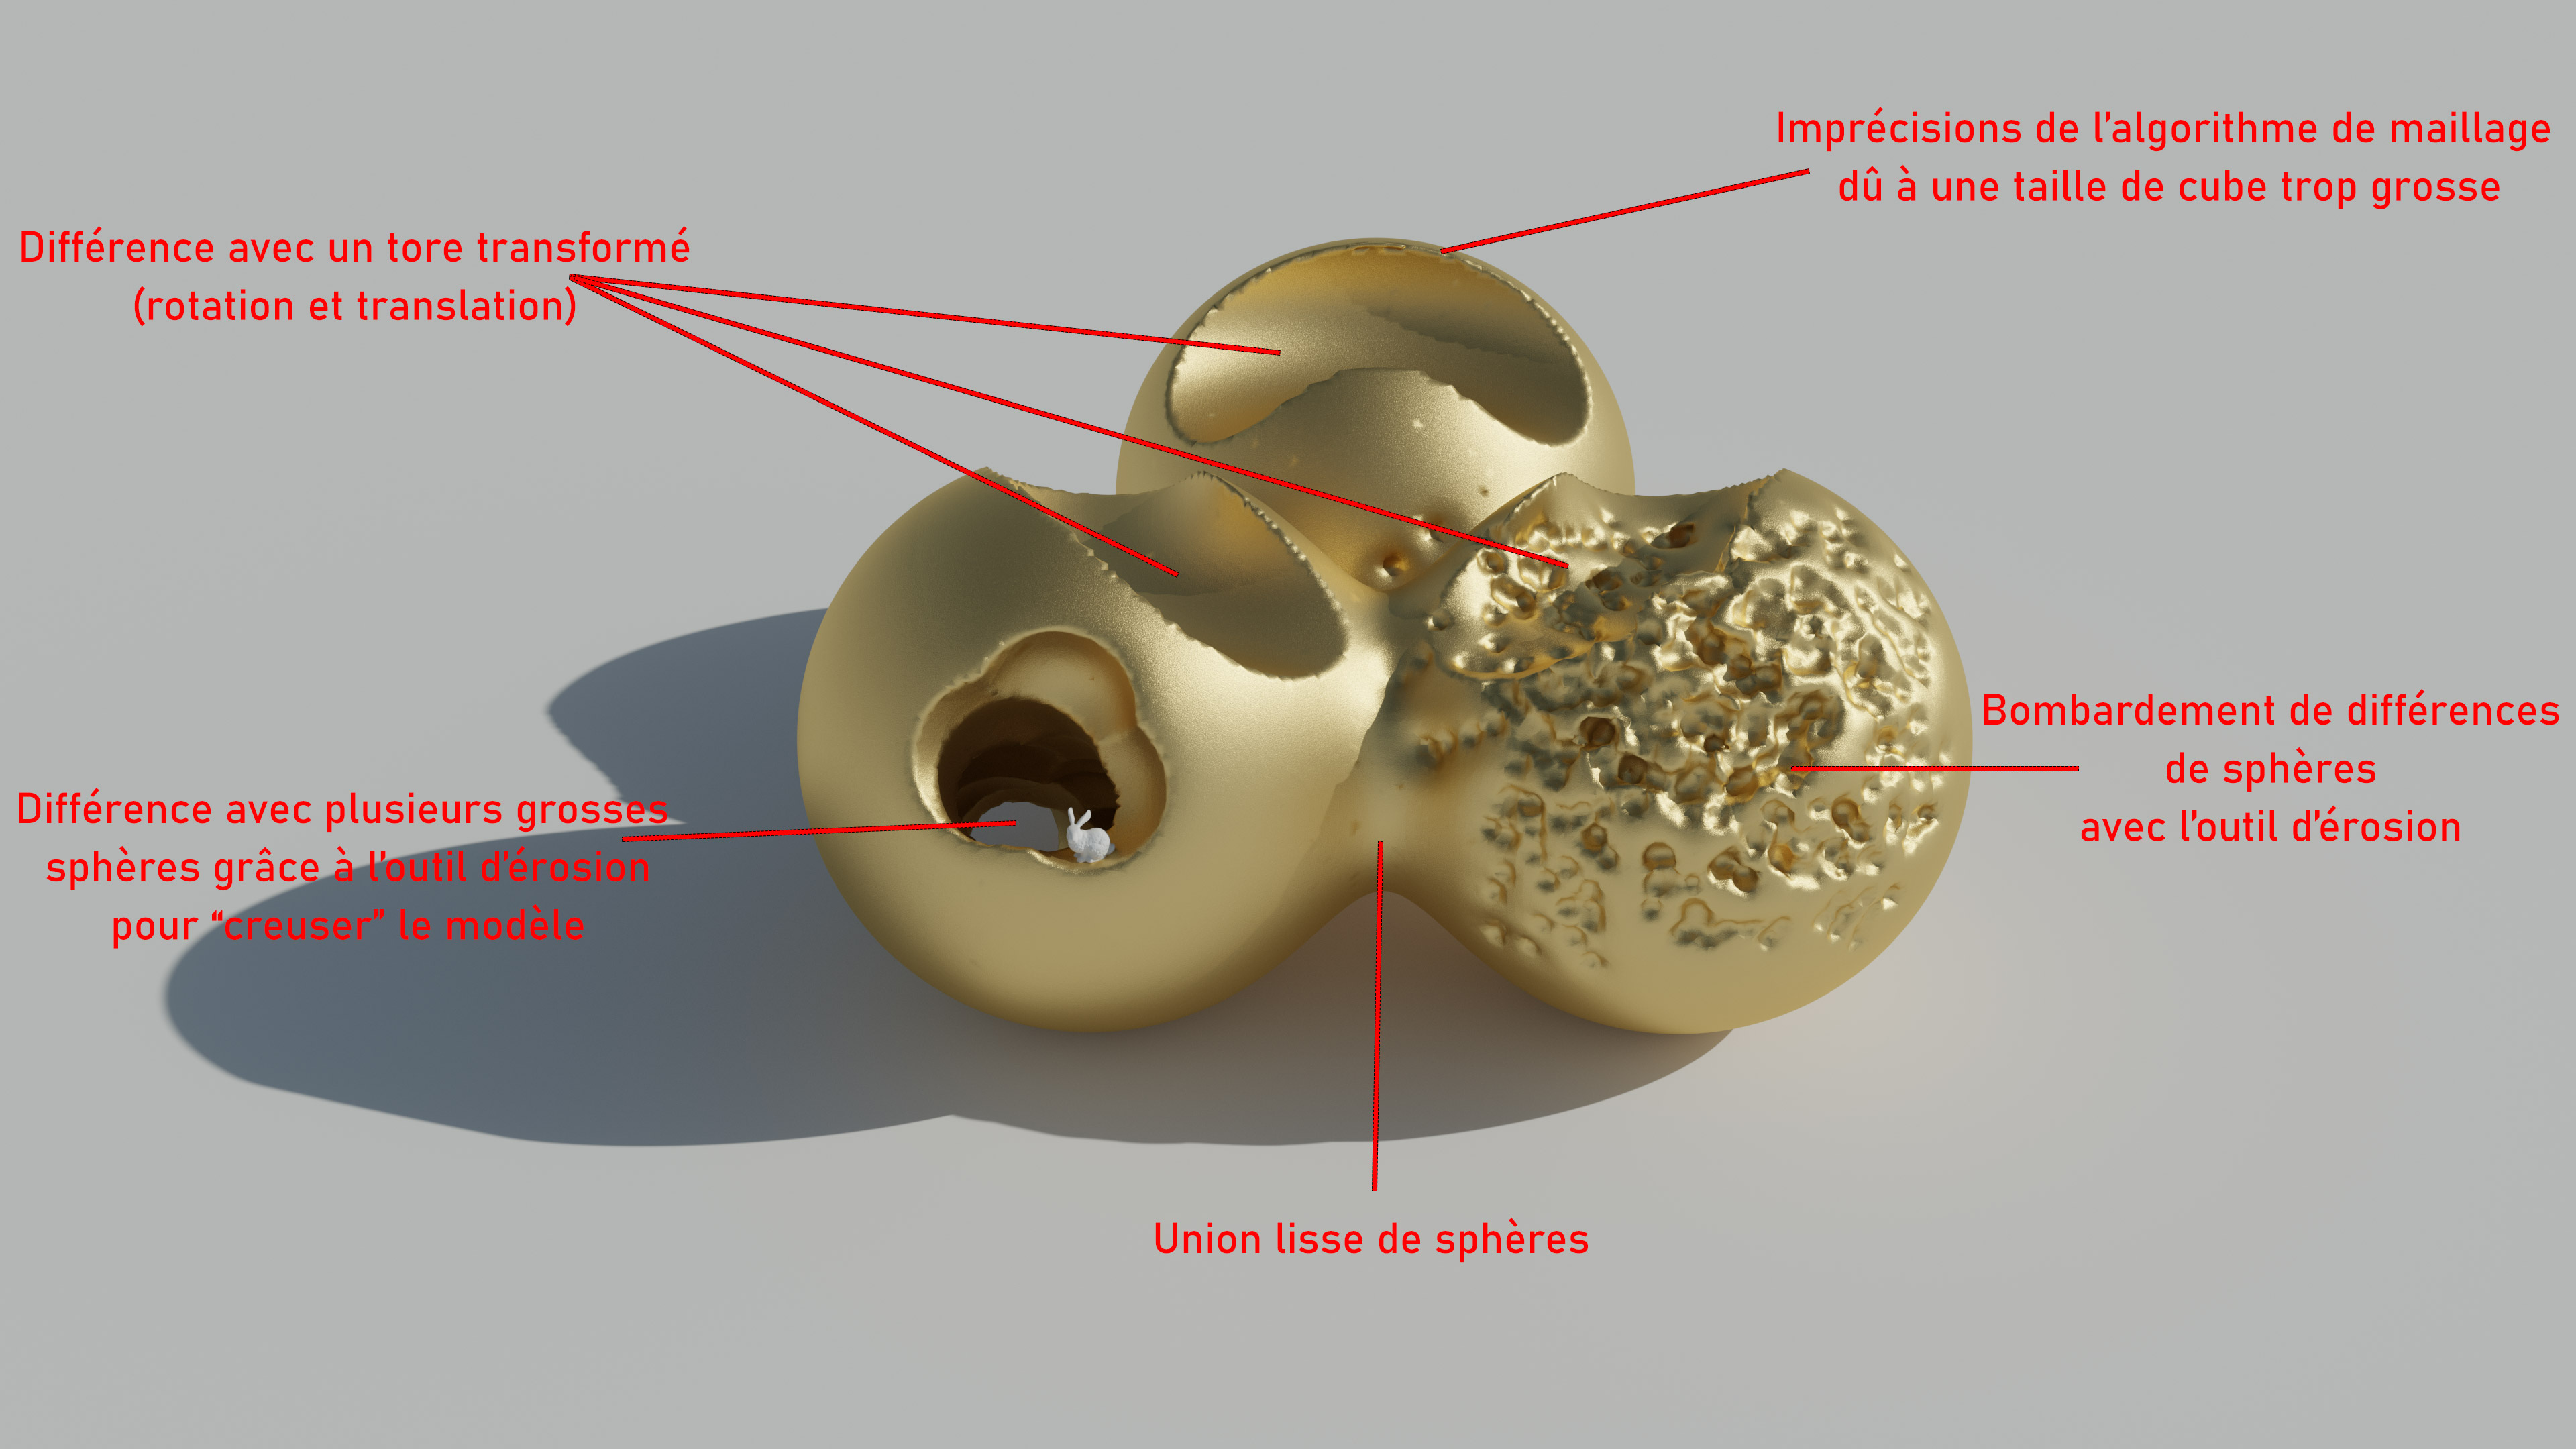
\includegraphics[width=1.2\textwidth]{Captures/Rendu.jpg}}

	\caption{Rendu Blender d'une surface implicite modélisée et maillée avec TinyMesh}
\end{figure}
\FloatBarrier

La modélisation par surface implicite permet la création de modèles très complexes mais le temps nécessaire ou maillage (ou au rendu par ray-marching) du modèle
dépend directement de la complexité du modèles / de l'arbre de construction. Pour ce TP, le plus gros consommateur de temps de calcul est l'outil d'érosion qui rajoute 
10 unions de sphères (ou plus) à la SDF. Chaque appel à la fonction \textit{Value()} de la SDF doit alors prendre en compte toutes ces nouvelles sphères.

\begin{figure}[h!]
	\adjustbox{center}{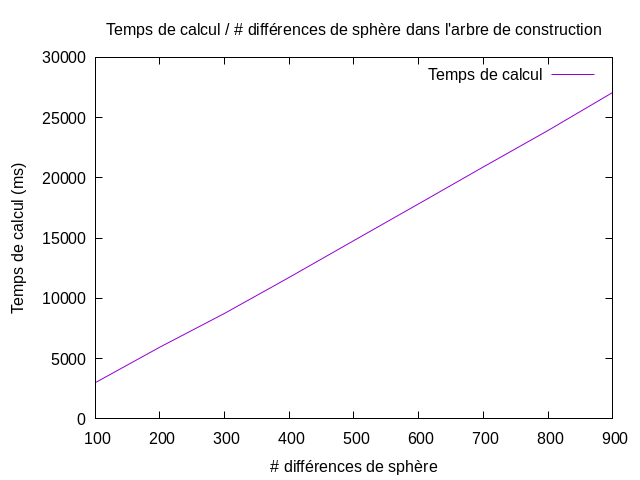
\includegraphics[width=0.8\textwidth]{Benchmark/remesh.png}}

	\caption{Temps d'exécution de l'algorithme de maillage de la surface implicite en fonction de la complexité de la SDF (nombre de différences de sphère utilisé dans la SDF)}
\end{figure}
\FloatBarrier

\subsection {Outil d'érosion}

L'outil d'érosion a été implémenté grâce à un algorithme de ray marching. On lance des rayons aléatoirement autour de la position où l'utilisateur a cliqué
et on rajoute des différences de sphère à la SDF aux points d'intersection. 

L'algorithme de ray marching faisant appel à la fonction \textit{Value()} de la SDF, il est de moins
en moins efficace (linéairement) au fur et à mesure que la SDF se complexifie. Un lancer de rayons + BVH sur le maillage de la surface implicite se révèle être 3 ordres de grandeur
plus rapide mais cela nécessite cependant d'avoir maillé la surface implicite au préalable.
